\begin{block}{Problem Statement}
  Maya has a single credit card with a credit limit of \$5,000. Her current statement balance is \$1,250.

  Calculate Maya's current credit utilization ratio. Is it within the common guideline of staying below 30\%?
\end{block}

\vspace{0.8em}
\centering
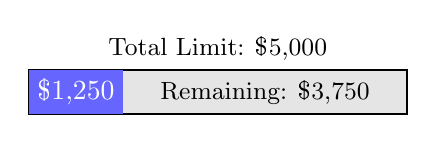
\begin{tikzpicture}[scale=0.8]
  % Visualizing balance vs limit
  \draw[thick, fill=gray!20] (0,0) rectangle (6,0.7);
  \fill[blue!60] (0,0) rectangle (1.5,0.7);
  \node at (0.75,0.35) {\color{white}\$1,250};
  \node at (3.75,0.35) {\small Remaining: \$3,750};
  \node[above] at (3,0.7) {\small Total Limit: \$5,000};
\end{tikzpicture}
